% !TeX program = lualatex 
\documentclass{mlai-report}

\usepackage[backend=biber,style=alphabetic, sorting=ynt]{biblatex} 
\renewcommand*{\nameyeardelim}{\addcomma\space}

%Use marginnotes to display the authors of the sections
\usepackage{marginnote}
\renewcommand*{\marginfont}{\normalcolor\normalfont\small} 


\usepackage{csquotes} 

%Nice and easy references
\usepackage{varioref}
\usepackage{cleveref}
 
% Please change this according to your situation
\title{Lab - Machine learning on encrypted data:\\ Logistic Regression implementation with CKKS} 
\author{Van Thong Nguyen (VTN) \and Gerd Mund (GM) \and Yat Wai Wong (YWW)}
\date{\today} 


\addbibresource{references.bib} 
\usepackage{blindtext} 
\usepackage{chngcntr}
\usepackage{placeins}
\counterwithout{table}{section}
\usepackage{subcaption}
\usepackage{float}
\usepackage{array}
\usepackage{graphicx,wrapfig,lipsum}
\usepackage{amsthm}
\usepackage{graphics}
\usepackage{algorithm} 
\usepackage{algpseudocode} 
\usepackage{enumitem}
\usepackage{hyperref}
\usepackage[figure]{hypcap}
\usepackage[toc,page]{appendix}
\usepackage{biblatex}
\usepackage{algpseudocode}
\usepackage{algorithm}
\usepackage{amsfonts}
\usepackage{multirow}
\usepackage[section]{placeins}

\algnewcommand\algorithmicforeach{\textbf{for each}}
\algdef{S}[FOR]{ForEach}[1]{\algorithmicforeach\ #1\ \algorithmicdo}

\theoremstyle{definition}
\newtheorem{definition}{Definition}[section]

\begin{document}
	\maketitle
    \pagenumbering{roman}
    	\begin{abstract}\marginnote{VTN}
        In homomorphic encryption world, the Cheon-Kim-Kim-Song (CKKS) scheme is current\-ly known as the most efficient homomorphic encryption scheme for approximate arithmetic. It allows approximate addition and multiplication of encrypted real complex numbers \linebreak \cite{cheon2017homomorphic}. The fact that the encryption scheme can achieve practical performance in some applications, we evaluate logistic regression model with the CKKS scheme against encryption performance, training performance, and accuracy of the output model.   
        
        Currently, there are two well-known libraries which are built on top of the CKKS scheme: HEAAN (C++), and TenSEAL (Python). We decide to use TenSEAL, because the Python programming language is more accessible than C++ and it is popular in data science world. To begin with, we implement the logistic regression CKKS and run it on four randomly generated datasets: 
        \begin{itemize}[nosep]
            \item[-] \texttt{framingham} (40000 9-D points)
            \item[-] \texttt{LogReg\_sample\_dataset} (1000 2-D points)
            \item[-] \texttt{HRF\_samples\_small} (1000 5-D datapoints)
            \item[-] \texttt{HRF\_samples\_big}: (50000 5-D points)
        \end{itemize}
        In addition, we run a plain logistic regression on those datasets. Then we compare the plain logistic regression and the CKKS logistic regression in terms of performance, e.g., runtimes and accuracy of the final results. In conclusion, we find that difference between CKKS logistic regression's accuracy and the plain logistic regression's one is insignificant. However, the vector-by-vector training on CKKS encrypted dataset does take much more time, because the TenSEAL library does not support encrypted matrix addition and matrix multiplication at the time of the evaluation. 
        
        Besides the performance evaluation, we propose a solution to reduce the runtime and the amount of allocated memory drastically when encrypting the datasets with the CKKS scheme by packing multiple datapoints into a single datapoint. Finally, we also suggest a method to enable the CKKS logistic regression to deal with the packed datapoints.
    \end{abstract}
    \newpage
	\tableofcontents
	\newpage
	\pagenumbering{arabic}
	\section{Introduction}\marginnote{VTN}
    \begin{text}
    Nowadays, data encryption helps us with protecting our data from being leaked or stolen. However, at the very beginning of data encryption, it was impossible to compute with encrypted data. It raises a problem for companies and organizations which want to gain useful information from their customers' data and have to ensure the privacy regulations at the same time. This is where fully homomorphic encryption plays its part to enable, for example, arithmetic operations over the encrypted data. Therefore, the fully homomorphic encryption allow us to apply some machine learning algorithms to homomorphic encrypted data. 
    
    In this report, we would like to use the Cheon-Kim-Kim-Song fully homomorphic encryption scheme (CKKS) along with logistic regression to evaluate performance of training process and accuracy of generated models. Alternatively, the Brakerski/Fan-Vercauteren fully homomorphic encryption scheme (BFV) \cite{fan2012somewhat} could be an option. Nevertheless, it can only do arithmetic calculations over integers, which means we need to transform the data before processing. In contrast to BFV, CKKS is designed to deal with real numbers. As a result, we choose CKKS over BFV. The theory behind CKKS is explained in detail in the paper \textit{"Homomorphic Encryption for Arithmetic of Approximate Numbers"} \cite{cheon2017homomorphic}. This report will answer following questions: \textit{how is the performance of logistic regression over CKKS encrypted datasets, i.e. How fast is it to train the CKKS encrypted data compared with training plaintext data? Does logistic regression over CKKS encrypted datasets consume more memory than plain logistic regression does? How accurate is the final model of logistic regression over CKKS encrypted dataset?}

    In order to finalize the evaluation, four 2-class datasets are used for evaluating:
    \begin{itemize}[nosep]
        \item[-] \texttt{framingham} (40000 9-D points),
        \item[-] \texttt{LogReg\_sample\_dataset} (1000 2-D points),
        \item[-] \texttt{HRF\_samples\_small} (1000 5-D datapoints),
        \item[-] \texttt{HRF\_samples\_big}: (50000 5-D points).
    \end{itemize}
    Then the encrypted datasets are trained by using gradient-descent logistic regression. Measurements are taken on a single machine to prevent bias and any inconsistencies. 
    
    In addition, we would like to propose a method to reduce amount of memory needed to encrypt the data by CKKS scheme. The method also saves network bandwidth, if the encrypted data needs to be transferred over the network, i.e., the internet.
    \end{text}
    \section{Preliminaries}
    \subsection{Lattice-Based Cryptography} \marginnote{YWW}
    Lattice-based cryptography is compelling for the following reasons:
    \begin{itemize}
        \item \textbf{Post-quantum security:} Many lattice-based problems are conjectured to be hard for both classical and quantum adversaries, making lattice-based cryptography one of the candidates in NIST's post-quantum cryptography standardization process \cite{nist_pqc}.
        \item \textbf{Enables advanced cryptographic schemes:} Lattice-based cryptography provides a rich algebraic structure, thereby enabling the construction of advanced cryptographic schemes, e.g., fully homomorphic encryption \cite{BGV} \cite{bfv1} \cite{bfv2}, homomorphic signatures \cite{hsig}, and functional encryption \cite{FE}. Until very recently, lattice-based cryptography
        provided the only such realizations of these advanced schemes.
        \item \textbf{Security based on worst case hardness:} Cryptography typically based the security on average case hardness, which is a stronger requirement compared with average case hardness. However, lattice-based cryptography allows us to base security on average case hardness: Some results \cite{av1} \cite{av2} \cite{av3} \cite{av4} \cite{av5} show that certain problems (e.g. LWE, SIS problem, and their ring and module variants) are hard on average case, provided that the closely related lattice problems, e.g. approximate SVP, SIVP, are hard in the worst case. Thus, schemes based on these problems are secure unless all instances of those lattice problems are solvable in polynomial time.
    \end{itemize}
    \subsection{Learning with Errors (LWE) Problem} \marginnote{YWW}
    The Learning with Errors (LWE) problem is a cornerstone of modern lattice-based cryptography. It was introduced by Regev \cite{av1} and its hardness is based on certain assumptions regarding the worst-case hardness of standard lattice problems such as GAPSVP (the decision version of the shortest vector problem) and SIVP (the shortest independent vectors problem) \cite{Reg05, Pei09a}.
    
    \begin{definition}[LWE Distribution]
        Let $n \ge 1$ be the security parameter (dimension), $q \ge 2$ be a modulus, and $\chi$ be an error distribution over $\mathbb{Z}_q$. For a secret vector $\mathbf{s} \in \mathbb{Z}_q^n$, the LWE distribution $A_{\mathbf{s}, \chi}$ over $\mathbb{Z}_q^n \times \mathbb{Z}_q$ is sampled by choosing a vector $\mathbf{a} \in \mathbb{Z}_q^n$ uniformly at random, sampling an error $e$ from the distribution $\chi$, and outputting the pair $(\mathbf{a}, b = \langle \mathbf{a}, \mathbf{s} \rangle + e) \in \mathbb{Z}_q^n \times \mathbb{Z}_q$.
    \end{definition}
    \noindent The LWE problem has two primary forms: the search version and the decision version. The goal of the search problem is to recover the secret vector from given LWE samples. The decision problem, on the other hand, is to distinguish LWE samples from uniformly random ones. These problems are parameterized by the number of samples, $m$, which we usually take to be large enough that the secret is uniquely defined with high probability.
    \begin{definition}[Search LWE Problem]
    Given $m$ independent samples $(\mathbf{a}_i, b_i) \in \mathbb{Z}_q^n \times \mathbb{Z}_q$ drawn from $A_{\mathbf{s},\chi}$ for a uniformly random secret $\mathbf{s} \in \mathbb{Z}_q^n$ (fixed for all samples), the goal of the \textbf{search LWE problem}, denoted $\text{Search-LWE}_{n,q,\chi,m}$, is to find $\mathbf{s}$.
    \end{definition}

        \begin{definition}[Decisional LWE Problem]
    Given $m$ independent samples $(\mathbf{a}_i, b_i) \in \mathbb{Z}_q^n \times \mathbb{Z}_q$, where every sample is distributed according to either: (1) $A_{\mathbf{s},\chi}$ for a uniformly random $\mathbf{s} \in \mathbb{Z}_q^n$ (fixed for all samples), or (2) the uniform distribution, the goal of the \textbf{decisional LWE problem}, denoted $\text{Decision-LWE}_{n,q,\chi,m}$, is to distinguish which is the case with non-negligible advantage.
    \end{definition}

    \subsection{Ring Learning with Errors (RLWE) Problem} \marginnote{YWW}
    The Ring Learning with Errors (RLWE) problem, introduced by Lyubashevsky, Peikert, and Regev \cite{idealLatticeRLWE}, is an algebraic variant of LWE that provides significant efficiency improvements. Instead of working with vectors of integers, RLWE operates over polynomial rings, which allows for more compact ciphertexts and faster computations. The security of many modern cryptographic schemes, e.g. the fully homomorphic encryption scheme used in this lab (CKKS scheme \cite{cheon2017homomorphic}), is based on the hardness of the RLWE problem.
    \begin{definition}[Cyclotomic Ring]
    Let $\Phi_M(X)$ be the $M$-th cyclotomic polynomial of degree $N$. Let $\mathcal{R} = \mathbb{Z}[X]/\Phi_M(X)$ be the integer ring and write $\mathcal{R}/q \mathcal{R}$ as the residue ring of $\mathcal{R}$ modulo an integer $q$.\\
    In the CKKS scheme, polynomial with a power-of-two-degree is used, and $M$ is always twice that degree, i.e. the ring used in CKKS scheme is $\mathcal{R} = \mathbb{Z}[X]/(X^N + 1)$ and $N = M/2$.\\
    For an integer polynomial $a \in \mathcal{R} = \mathbb{Z}[X]/\Phi_M(X)$, the canonical embedding $CE(a)$ is $(a(\zeta_{M}^j)) \in \mathbb{C}^N$ where $0 < j < M$, $j \in \mathbb{Z}_M^\times$ and $\zeta_M = e^{2\pi i / M}$ is the primitive $M$th root of unity.
    \end{definition}
    
    \begin{definition}[Gaussian Distribution]
    For a real number $r$, we define the the Gaussian function as $\rho _r = \text{exp}(-\pi ||\mathbf{z}||^2 /r^2)$, where $||\mathbf{z}||$ is the $L_{2}$ norm of the vector $\mathbf{z}$.
    As a discrete Gaussian distribution is usually used as the RLWE error distribution, the continuous Gaussian distribution $\Psi_\mathbf{r}$ has to be discretized by a rounding function to the nearest integer, i.e. $\lfloor \Psi_\mathbf{r} \rceil$.
    \end{definition}

    \begin{definition}[RLWE Distribution]
Here, we define the (decisional) RLWE distribution as follows. We use the dual  $\mathcal{R}^{\lor} = N^{-1} \cdot \mathcal{R}$ as the fractional ideal of $\mathcal{R}$ and $\mathcal{R}^\lor_q = \mathcal{R}^\lor/q\mathcal{R}^\lor$. For a secret $s \in \mathcal{R}_q^\lor$, let $q \geq 2$ be the modulus,  $\mathbf{r} \in (\mathbb{R}_{>0}) ^N$ and an error distribution $\chi := \lfloor \Psi_\mathbf{r} \rceil_{\mathbb{R}^{\lor}}$, a RLWE distribution $A_{N,q,\chi}(s)$ over $\mathcal{R}_q \times \mathcal{R}_q^\lor$ is sampled by choosing $a \leftarrow \mathcal{R}_q$ uniformly at random, $e \leftarrow \chi$, and output an RLWE instance as $(a, a \cdot s + e) \in \mathcal{R}_q \times \mathcal{R}_q^\lor$\footnote{Note that the form of RLWE sample is sometimes written as $(a, a \cdot s + e) \in \mathcal{R}_q \times \mathcal{R}_q^$. The RLWE problems in these two forms are entirely equivalent in terms of computation, but it turns out that  $\mathcal{R}_q \times \mathcal{R}_q^\lor$ form is the right definition for hardness proof and cryptographic applications when using a (nearly) spherical error $e$ \cite {idealLatticeRLWE} \cite{toolkitRLWE}. To obtain this form of RLWE instance, $s, (a \cdot s + e) \in \mathcal{R}_q^\lor$ can be transformed by multiplying them by a tweak factor $t$, such that $ts, (a \cdot ts + te) \in \mathcal{R}_q$ and $(a, a \cdot ts + te) \in \mathcal{R}_q \times \mathcal{R}_q^$. As CKKS scheme uses a power-of-two cyclotomic ring, the dual is $\mathcal{R}^{\lor} = N^{-1} \cdot \mathcal{R}$. Thus the tweak factor for $s$ and $e$ is just $N$.}.
\end{definition}
\begin{definition}[Search RLWE Problem]
The \textbf{search RLWE problem} is to recover the secret $s$ from a given set of samples from the RLWE distribution $A_{N,q,\chi}(s)$.
\end{definition}
\begin{definition}[Decisional RLWE Problem]
The decisional RLWE problem is to distinguish between the samples drawn from the RLWE distribution $A_{N,q,\chi}(s)$ and the samples drawn uniformly at random from the distribution $\mathcal{R}_q \times \mathcal{R}_q^\lor$, with non-negligible probability.
\end{definition}

\subsection{Module Learning with Errors (MLWE) Problem} \marginnote{YWW}
The Module Learning with Errors (MLWE) problem is a generalization of the LWE and RLWE problem. It offers a flexible trade-off between the efficiency of RLWE and the generality of LWE. Instead of working with single polynomials in a ring $\mathcal{R}$, MLWE operates on modules over the ring $\mathcal{R}$, which are essentially vectors of ring elements.
\begin{definition}[MLWE Distribution]
Let $k, d \ge 1$ be dimensions, $\mathcal{R}_q$ be a polynomial ring modulo $q$ (e.g. $\mathcal{R}_q = \mathbb{Z}_q[X]/(X^d + 1)$), and $\chi$ be an error distribution over $\mathcal{R}_q$. For a secret vector $\mathbf{s} \in \mathcal{R}_q^k$, the MLWE distribution $A_{\mathbf{s}, \chi}$ is sampled by choosing a vector $\mathbf{a} \in \mathcal{R}_q^k$ uniformly at random, sampling an error $e \leftarrow \chi$, and outputting the pair $(\mathbf{a}, b = \langle \mathbf{a}, \mathbf{s} \rangle + e) \in \mathcal{R}_q^k \times \mathcal{R}_q$.
\end{definition}
\noindent Using $\mathbb{Z}_q$ as the $\mathcal{R}_q$ in the MLWE definition obtains the plain LWE definition. On the other hand, setting $k=1$ obtains the RLWE definition.
\begin{definition}[Search MLWE Problem]
Given a set of samples from the MLWE distribution, the \textbf{search MLWE problem} is to recover the secret vector $\mathbf{s}$.
\end{definition}

\begin{definition}[Decisional MLWE Problem]
The \textbf{decisional MLWE problem} is to distinguish between samples from the MLWE distribution and uniformly random samples from $\mathcal{R}_q^k \times \mathcal{R}_q$.
\end{definition}

    \subsection{Fully Homomorphic Encryption and Bootstrapping} \marginnote{YWW}
    Fully homomorphic encryption is an encryption scheme that enables computation on encrypted data and produces encrypted results matching those of plaintext computations, without needing to decrypt the data to know the decryption key. More precisely, one can take a set of encrypted message \textsf{Enc}$(x_1),...,$\textsf{Enc}$(x_n)$ and  homomorphically compute a function on this set, i.e.  produce an encryption of the function of them, that is, \textsf{Enc}$(f(x_1,...,x_n))$. The homomorphic computation is correct, i.e. 
    \[
    \textsf{Dec}_{sk}(\textsf{Enc}_{pk}(f(x_1,...,x_n))) = f(x_1,...,x_n).
    \]
    Homomorphic encryption schemes built from LWE usually have a problem of error growth from homomorphic computations, which makes the scheme being not able to compute functions correctly after the error grows to a certain size. These schemes can only homomorphically evaluate a circuit of a bounded depth, and they are usually called `somewhat homomorphic' or `leveled homomorphic'.\\
    A concept called `bootstrapping' proposed by Gentry \cite{bootstrapping} allows us to reduce the error rate of a ciphertext, thus enables homomorphic computation with unbounded depth. Such an encryption scheme with unbounded depth is called fully homomorphic encryption. Suppose we have a ciphertext $C$ of the plaintext $m$, where its error rate is too large for a further homomorphic operation. The idea behind bootstrapping is to encrypt the secret key, i.e. $\textsf{Enc}(sk)$, then homomorphically evaluate the decryption function on $C$ and $\textsf{Enc}(sk)$. Thus, the homomorphic decryption function $\textsf{Dec}_{HE}$ will produce a `refreshed' ciphertext $C'$, which is the encryption of $m$ with a lower error rate:
    \[
    \textsf{Dec}_{HE}(\textsf{Enc}(sk), C) = C', \textsf{Dec}(C') = m.
    \]
    \subsection{Cheon-Kim-Kim-Song homomorphic encryption scheme} \marginnote{YWW}
    The CKKS scheme is a fully homomorphic encryption scheme for approximate arithmetic, which supports approximate addition and multiplication on real numbers with unbounded depth. Its security is based on the hardness to solve the ring learning with errors problem (RLWE), and the decryption of this scheme results in a small error on data, which is acceptable for some real world applications.\\
    \\
    \textbf{Batching and plaintext encoding.} 
    The idea of batching in FHE scheme is to batch multiple plaintexts into a single ciphertext, which allows us to perform homomorphic computation efficiently with parallel computation. As the CKKS scheme relies on RLWE, the batched vectors must be encoded into polynomials contained in an appropriate cyclotomic ring. The idea of encoding and decoding is to use the canonical embedding, e.g.\@{} a plaintext vector $\mathbf{z} \in \mathbb{C}^{N/2}$ is encoded as a polynomial $m(X) \in \mathbb{Z}[X]/(X^N +1)$ by the inverse of canonical embedding and vice versa. \\
    More precisely, the image of the canonical embedding is in the subring $\mathbb{H} = \{(z_j)_{j \in \mathbb{Z}_M^{\times}}: z_j = \overline{z_{-j}} \}$ of  $\mathbb{C}^N$. As half of the elements in $\mathbb{H}$ are conjugate to the other half, the plaintext vectors $\mathbf{z}$ are in $\mathbb{C}^{N/2}$. To project from $\mathbb{C}^{N}$ to $\mathbb{C}^{N/2}$, a projection $\pi$ is defined by $(z_j)_{j \in \mathbb{Z}_M^{\times}} \mapsto (z_j)_{j \in T}$ where $T$ is a multiplicative subgroup of $\mathbb{Z}_M^{\times}$ satisfying $\mathbb{Z}_M^{\times} / T = \{ \pm 1\}$.\\
    In the encoding algorithm, we first need to expand vector $\mathbf{z} \in \mathbb{C}^{N/2}$ to $\mathbb{C}^{N}$ by using $\pi^{-1}$.  As $CE(\mathcal{R})$ is countable but $\mathbb{H}$ is isomorphic to $\mathbb{C}^{N/2}$ (defined by $\pi$) and uncountable, $\pi^{-1}(\mathbf{z})$ may not be in  $CE(\mathcal{R})$. Thus we need to discretize $\pi^{-1}(\mathbf{z})$ by the coordinate-wise randomized rounding (written as $\lfloor\,\,  \rceil_{CE(\mathcal{R})}$) \cite{toolkitRLWE}. \\
    As rounding in encoding process may destroy some significant figures, we need to multiply the plaintext by a scaling factor $\Delta$ before encoding, and divide it by $\Delta^{-1}$ in the decoding algorithm. \\
    The full encoding and decoding algorithm are defined as follows: 
    \begin{itemize}
    \item Encoding: a vector $\mathbf{z} \in \mathbb{C}^{N/2}$ is taken as input. We first expand it to $\pi^{-1}(\mathbf{z}) \in \mathbb{H}$, then multiply it by the scaling factor $\Delta$, followed by the rounding function. Finally, apply the inverse of canonical embedding $CE^{-1}$. The resulting polynomial is$$m(X) = CE^{-1}(\lfloor\Delta\cdot\pi^{-1}(\mathbf{z})\rceil_{CE(\mathcal{R})} \in \mathcal{R}$$
    \item Decoding: a polynomial $m \in \mathcal{R}$ is taken as input. The resulting vector is $$z = \pi \circ CE(\Delta^{-1}\cdot m) \in \mathbb{C}^{N/2}$$
    \end{itemize}
    \textbf{Encryption and decryption.} In the CKKS scheme, the encryption of a plaintext $m$ outputs $(c_0, c_1) = (-a \cdot s + e + m, a) \mod q$, and the decryption of a ciphertext is $\textsf{Dec}_s(c_0, c_1) = c_0 + c_1 \cdot s = (-a \cdot s + e + m) + a \cdot s = m + e \mod q$.\\
    \\
    \textbf{Bootstrapping.} As the decryption algorithm consists of a modular reduction, the bootstrapping of CKKS scheme thus includes a homomorphic modular reduction. Since CKKS scheme is infeasible to do homomorphic modular reduction, Cheon et al. \cite{10.1007/978-3-319-78381-9_14} proposed a bootstrapping for CKKS scheme where the  decryption formula is approximated by an approximate polynomial of a scaled sine function. A trigonometric function is a good approximation of modular reduction because it is the identity near zero and periodic with period $q$. \\
    \\
    \subsection{Logistic Regression} \marginnote{YWW}
    Logistic regression is a common supervised machine learning model mainly for two-class classification. Consider an observation $x$ with features $[x_1, x_2,...,x_n]$ and it can be classified as one of the two classes, the main idea of logistic regression is to apply the learned parameters (weights and bias) to the features, then uses the logistic sigmoid function as the classifier to classifies that observation as one of the two classes (A real world example can be a spam filter classifying an email as `spam' or `not spam'). Weights $w_i$ are real numbers which represent how important the features $x_i$ is to the classification. \@{}Bias $b$, also called intercept, is another real number which is added to the weighted features. Applying weights and bias to the features means:
    \[
    \left(\sum_{i = 1}^{N}w_ix_i \right) + b
    \]
    We simplify the above notation with $w_0 = b$ and $x_0 = 1$:
    \[
    \left(\sum_{i = 0}^{N}w_ix_i \right)
    \]
    Logistic sigmoid function is used as the classifier of logistic regression. The function has the form
    \[
    \sigma(a) = \frac{1}{1 + \exp(-a)}
    \]
    and always maps to a range of $[0, 1]$, which can be used as the probability of an observation being classified as a certain class. The term `sigmoid' means S-shaped, as you can see in figure \ref{fig:LR}. This type of function is usually called `squashing function' because it maps the whole real axis into a finite interval. 
       \begin{figure}[ht]
        \centering
        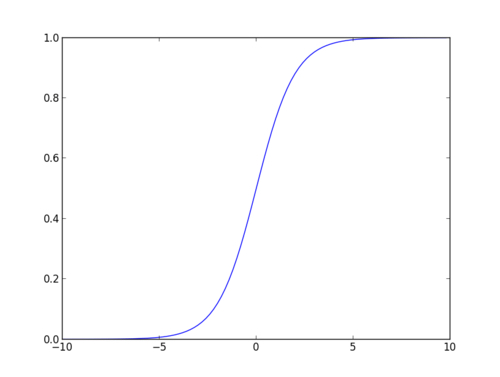
\includegraphics[width=0.5\linewidth]{images/LR.jpg}
        \caption{Plot of the logistic sigmoid function}
        \label{fig:LR}
    \end{figure} 
    As CKKS scheme can only evaluate polynomial function, the logistic sigmoid function can only be approximated by a specific polynomial. Refer to section 3.1 for details.\\
    \\
    To use the sigmoid function as the classifier, we apply the function to the weighted features. Suppose the two classes of our data set are $\textcal{C}_0, \textcal{C}_1$, $\mathbf{x}$ is the feature vector of an observation and $\mathbf{w}$ is the weight vector, the probability of that observation classified as  $\textcal{C}_0$ is
    \[
    prob.(\text{label} = \textcal{C}_0 | \mathbf{x}) = \sigma(\mathbf{w}^T\mathbf{x}) = \frac{1}{1 + \exp(-\mathbf{w}^T\mathbf{x})}
    \]
    and the probability for the other class is 
     \[
    prob.(\text{label} = \textcal{C}_1 | \mathbf{x}) = 1 - \sigma(\mathbf{w}^T\mathbf{x}) = 1 - \frac{1}{1 + \exp(-\mathbf{w}^T\mathbf{x})} = \frac{\exp(-\mathbf{w}^T\mathbf{x})}{1 + \exp(-\mathbf{w}^T\mathbf{x})}
    \]
    As the sigmoid funtion has the property:
    \[
    1 - \sigma(a) = \sigma(-a)
    \]
    we can express $prob.(\text{label} = \textcal{C}_1 | \mathbf{x})$ as $\sigma(-(\mathbf{w}^T\mathbf{x}))$.\\
    \\
    To optimise the accuracy of the classifier, logistic regression learns the weights and bias from the training data set at training phase, such that the classified classes are as close to the true classes as possible. We use gradient descent as our optimisation algorithm.
    \subsection{Optimisation Methods for Logistic Regression with CKKS} \marginnote{VTN}
   To optimise the accuracy of the model, nonlinear optimization methods are needed to estimate the regression parameters, i.e. weights and bias. The most well-known cost function optimization approaches in logistic regression are the Newton-Raphson method and the gradient descent method. Since matrix inversion is a must when using the Newton-Raphson method and the CKKS scheme does not support that feature, we put the Newton-Raphson method aside and consider the gradient descent method to train the encrypted datasets. Fortunately, the gradient descent method does not need matrix inversion and any division operations, as a result it is suitable for training the CKKS encrypted data.\\
   \subsection{Gradient Descent} \marginnote{YWW}
    Gradient descent is a common optimisation algorithm in machine learning to learn the model parameters. The main idea is to define a cost function (or error function) for the classifier, then iteratively update the parameters to go to the negative direction of the gradient of the error function at the current point until it goes to the local minimum.\\
       \begin{figure}[ht]
        \centering
        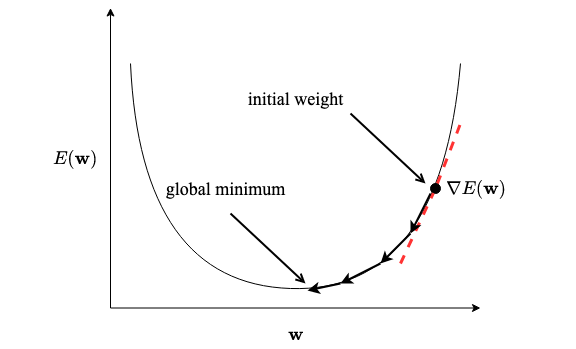
\includegraphics[width=0.8\linewidth]{images/gradient descent.png}
        \caption{Example of gradient descent which iteratively goes to the negative direction of the gradient until it reaches the local minimum (also global minimum in this example).}
        \label{fig:GD}
    \end{figure} 
    \\
    For a training data set $\{X, T\}$ with $N$ data points, we denote $x_i$ as the features of a single data point $i = 1,...,N$ and $t_i \in \{0, 1 \}$ is the true class. As the true classes are binary, the data set is a Bernoulli distribution. The probability or likelihood for a single data point is:
    \[
    prob.(t_i | x_i) = y_i^{t_i} (1 - y_i)^{1 - t_i}
    \]
    and the likelihood function for the data set is:
    \[
    prob.(T | X) = {\displaystyle \prod_{i=1}^{N} y_i^{t_i}(1 - y_i)^{1 - t_i}}
    \]
    where $y_i = \sigma(\mathbf{w}^T\mathbf{x})$ is the predicted value from the classifier. This probability represents how likely the true classes being classified. We then take the negative logarithm of the likelihood function as the error function:
    \[
    E(\mathbf{w}) = -\text{log}prob.(T|X) = {\displaystyle \sum_{i=1}^{N} (t_i \text{log}y_i + (1 - t_i)\text{log}(1 - y_i) )}
    \]
    This negative logorithm of the likelihood function represents how much the predicted classes differ from the true classes. We then need the gradient of the error function for the gradient descent method. The goal of gradient descent is to iteratively update the parameter of the model, i.e. the weight vector $\mathbf{w}$, until the gradient of the error function is in local minimum. Using the derivative to take the gradient of the error function, we get
    \[
    \nabla E(\mathbf{w}) = {\displaystyle \sum_{i=1}^{N} (y_i - t_i)x_i}
    \]
    This gradient of the error function is used for the iterative update of the weight as follows:
    \[
    \mathbf{w}^{\text{step } i+1} \leftarrow \mathbf{w}^{\text{step } i} - \alpha \nabla E(\mathbf{w})
    \]
    where $\alpha > 0$ is the learning rate. A higher learning rate means we adjust $\mathbf{w}$ more on each step, but it leads to the problem of overshooting the minimum of the error function. It is common to start with a higher learning rate then slowly decrease it.


    \section{Related Work}\marginnote{VTN}
    \begin{text}
    In this section, we would like to introduce two papers: \textit{Secure logistic regression Based on Homomorphic Encryption: Design and Evaluation} \cite{MiranKim2018}, and \textit{logistic regression model training based on the approximate homomorphic encryption} \cite{Kim2018}. Both of the papers present ways to implement logisctic regression based on the CKKS encryption scheme.
    \end{text}
    
    \subsection{Secure logistic regression Based on Homomorphic Encryption: Design and Evaluation}\marginnote{VTN}
    The authors adapted the CKKS encryption scheme which is optimized for real number computation. Notably, a least squares approximation of the logistic function is introduced to improve accuracy and efficiency.
    
    We know that the sigmoid function plays an important part in logistic regression data training using the gradient descent method. Despite the gradient descent can be used along with CKKS encryption scheme, there is still a computational difficulty during the implementation. The sigmoid function becomes that issue, because the CKKS can only evaluate the polynomial functions. Therefore, Taylor polynomials have been formulated as an approximate replacement of the sigmoid function. However, we found that even if the Taylor polynomial $T_9(x)$ is used, the accuracy is not enough; it is a local approximation near a certain point (see figure \ref{fig:approxsigmoid}a). 
    
    \begin{figure}[ht]
        \centering
        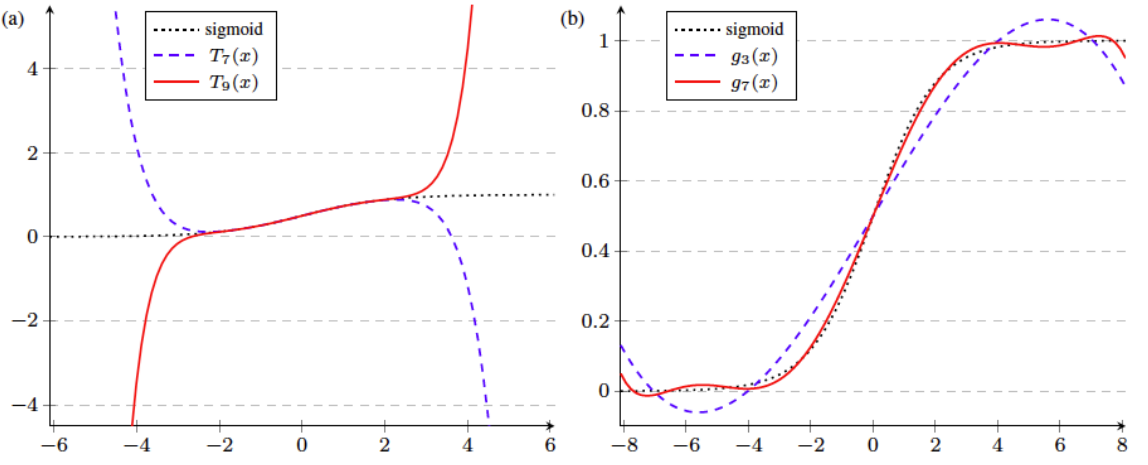
\includegraphics[width=1\linewidth]{images/Screenshot from 2021-10-03 23-12-29.png}
        $g_3(x)=0.5 + 1.20096 * (x/8) - 0.81562 * (x/8)^3$
        
        $g_7(x)=0.5 + 1.73496 * (x/8) - 4.19407 * (x/8)^3 + 5.43402 * (x/8)^5 - 2.50739 * (x/8)^7$
        \caption{Graphs of (a) sigmoid function and Taylor polynomials and (b) sigmoid function and least squares approximations. \cite{MiranKim2018}}
        \label{fig:approxsigmoid}
    \end{figure} 
    
    Due to limitation of the Taylor polynomial, Miran Kim at al. \cite{MiranKim2018} adopted a global approximation to minimize the the mean squared error which is defines by:
    $(1 / |I|) \int_{I}f(x)^2dx$, where $f(x)$ is an integrable function and $I$ is an interval. The least squares method is meant to produce a polynomial $g(x)$ of degree $d$ minimizing the mean squared error $(1 / |I|) \int_{I}(f(x) - g(x))^2dx$. The authors used degree 3 and 7 least squares approximation of the sigmoid function over the interval [-8,8] (see formulas in figure \ref{fig:approxsigmoid}). It has been proved that $g_3$ only needs a smaller depth for evaluation, while $g_7$ is more precise.

    \begin{text}
    In order to evaluate their method, five chosen datasets are described in table \ref{tab:miranDesOfData}. These single-binary-labeled datasets can be used to train binary classifiers, e.g., logistic regression. In table \ref{tab:miranCompare}, the final models of encrypted approach and encrypted logistic regression are compared. We see that the gaps between those models are not huge; therefore, the paper's approach is as good as the unencrypted logistic regression with the original sigmoid function. 
    \end{text}
    
    \begin{table}[ht]
        \centering
        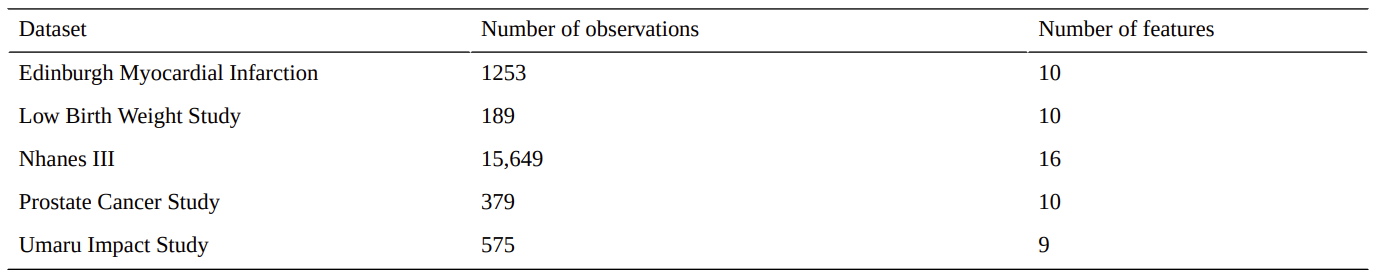
\includegraphics[width=1\linewidth]{images/Screenshot from 2021-10-03 23-53-36.png}
        \caption{Description of datasets. \cite{MiranKim2018}}
        \label{tab:miranDesOfData}
    \end{table} 
    
    \begin{table}[ht]
        \centering
        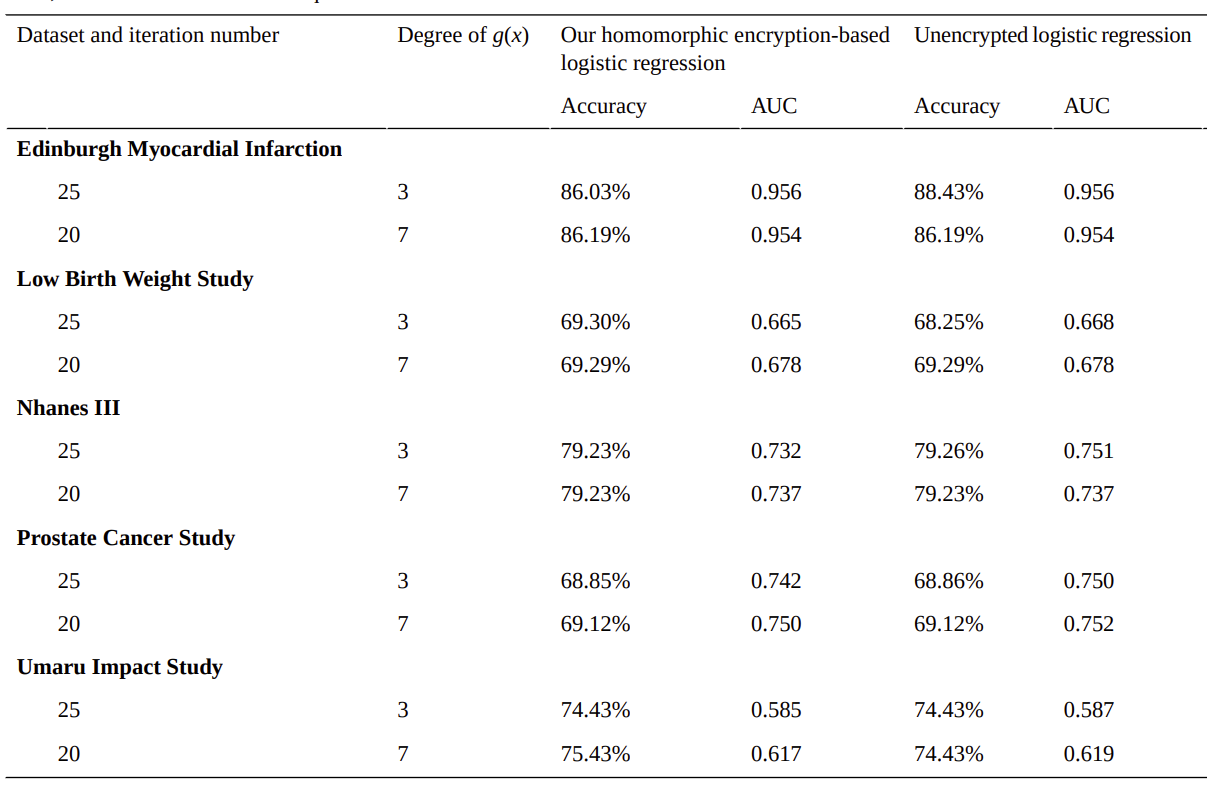
\includegraphics[width=1\linewidth]{images/Screenshot from 2021-10-04 00-12-26.png}
        \caption{Comparison of encrypted/unencrypted logistic regression. \cite{MiranKim2018}}
        \label{tab:miranCompare}
    \end{table} 
    
    \subsection{Logistic regression model training based on approximate homomorphic encryption}\marginnote{VTN}
    Similar to the papers of \cite{MiranKim2018}, \cite{Kim2018} also described a mean to train a logistic regression model without leaking any information by using the CKKS encryption scheme. Especially, they proposed a new encoding method to reduce the size of the encrypted database. In addition, adapting Nesterov's accelerated gradient descent helps to reduce the number of iterations as well as computational power while assuring the quality of final models.
    
    The Gradient Descent has an issue when dealing with the local minimas. If the learning rate is too low, we might stuck in a local minima; therefore, we cannot get to the global minima. Many gradient descent algorithms have been developed to overcome this problem, for example, momentum gradient descent. Nesterov Accelerated Gradient D`escent \cite{Nesterov} is a variant of momentum gradient descent. It applies moving average to the update vector, and calculate the gradient at this "look-ahead" position afterward. It is proved to give a better convergence of $O(1/t^2)$ after iterating $t$ steps theoretically as well as practically. The weight update equations of the Nesterov's accelerated gradient descent are shown in figure \ref{fig:nesteroveq}.
    
    \begin{figure}[ht]
        \centering
        $\theta^{(t+1)} \xleftarrow[]{} v^{(t)} - \alpha_t \cdot \nabla{J}(v^{(t)})$
    
        $v{(t+1)} \xleftarrow[]{} (1 - \gamma_t) * \theta^{(t+1)} + \gamma_t \cdot \theta^{(t)}$
        \caption{Equations of Nesterov Accelerated Gradient Descent. $0 < \gamma_t < 1$. $0 < \alpha_t < 1$}
        \label{fig:nesteroveq}
    \end{figure}
    
    In order to achieve an efficient computation, the authors pack all data points of a dataset into a single vector in row-by-row order. The concept is shown in figure \ref{fig:dataencodeconcept}; where each row represents one data point, $(f+1)$ is the number of features, and $n$ is the number of data points in the dataset. To evaluate gradient descent on the vector $w$, shifting operations of row and column vectors are needed. A shift algorithm \textit{Rot($w$, $r$)} can shift the encrypted vector $w$ by $r$ positions. For example, we get a new dataset $Z'$ (see figure \ref{fig:shiftedw}), if we do \textit{Rot($w$, $f+1$)} (which means we shift the vector $w$ by $(f+1)$ positions).
    
    \begin{figure}[ht]
	    \centering
	    \subfloat[][The dataset described as a matrix $Z$]{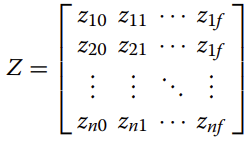
\includegraphics[width=0.3\linewidth]{images/Screenshot from 2021-10-04 01-48-54.png}\label{fig:matrixR}}\qquad
        \subfloat[][The matrix $Z$ is packed in a vector $w$]{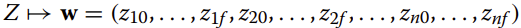
\includegraphics[width=0.47\linewidth]{images/Screenshot from 2021-10-04 01-49-05.png}\label{fig:vectorw}}
        \caption{Data encoding concept of paper \cite{Kim2018}} \label{fig:dataencodeconcept}
	\end{figure}
	
	\begin{figure}[ht]
        \centering
        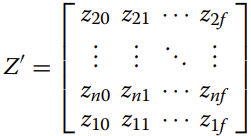
\includegraphics[width=0.3\linewidth]{images/Screenshot from 2021-10-04 02-04-49.png}
        \caption{New matrix $Z'$ corresponding to the shifted vector $w'$. Where $w'$ = \textit{Rot($w$, $f+1$)} \cite{Kim2018}}
        \label{fig:shiftedw}
    \end{figure} 
    
    Applying the Nesterov Accelerated Gradient Descent \cite{Nesterov} and the data packing approach above, we achieve similar output models as the approach described in \cite{MiranKim2018} with much less runtimes and less allocated memory. The results are shown in the table \ref{fig:comparetable}.
    
    \begin{table}
    \resizebox{\textwidth}{!}{\begin{tabular}{ c c c c c c c c c c c }
    \hline
    Dataset & Sample num & Feature num & Method & deg $g$ & Iter num & Enc time & Learn time & Storage & Accuracy & AUC\\
    \hline
    \multirow{3}{4em}{Edinburgh} & \multirow{3}{4em}{1253} & \multirow{3}{4em}{9} & \cite{Kim2018} & 5 & 7 & 2s & 3.6 min & 0.02 GB & 91.04\% & 0.958  \\ 
    &&& \cite{MiranKim2018} & 3 & 25 & 12s & 114 min & 0.69 GB & 86.03\% & 0.956 \\ 
    &&& \cite{MiranKim2018} & 7 & 20 & 12s & 114 min & 0.71 GB & 86.19\% & 0.954 \\ 
    \multirow{3}{4em}{lbw} & \multirow{3}{4em}{189} & \multirow{3}{4em}{9} & \cite{Kim2018} & 5 & 7 & 2s & 3.3 min & 0.02 GB & 69.19\% & 0.689  \\ 
    &&& \cite{MiranKim2018} & 3 & 25 & 11s & 99 min & 0.67 GB & 69.30\% & 0.665 \\ 
    &&& \cite{MiranKim2018} & 7 & 20 & 11s & 86 min & 0.70 GB & 69.29\% & 0.678 \\ 
    \multirow{3}{4em}{nhanes3} & \multirow{3}{4em}{15649} & \multirow{3}{4em}{15} & \cite{Kim2018} & 5 & 7 & 14s & 7.3 min & 0.16 GB & 79.22\% & 0.717  \\ 
    &&& \cite{MiranKim2018} & 3 & 25 & 21s & 235 min & 1.15 GB & 79.23\% & 0.732 \\ 
    &&& \cite{MiranKim2018} & 7 & 20 & 21s & 208 min & 1.17 GB & 79.23\% & 0.737 \\ 
    \multirow{3}{4em}{pcs} & \multirow{3}{4em}{379} & \multirow{3}{4em}{9} & \cite{Kim2018} & 5 & 7 & 2s & 3.5 min & 0.02 GB & 68.27\% & 0.740  \\ 
    &&& \cite{MiranKim2018} & 3 & 25 & 11s & 103 min & 0.68 GB & 68.85\% & 0.742 \\ 
    &&& \cite{MiranKim2018} & 7 & 20 & 11s & 97 min & 0.70 GB & 69.12\% & 0.750 \\ 
    \multirow{3}{4em}{uis} & \multirow{3}{4em}{575} & \multirow{3}{4em}{8} & \cite{Kim2018} & 5 & 7 & 2s & 3.5 min & 0.02 GB & 74.44\% & 0.603  \\ 
    &&& \cite{MiranKim2018} & 3 & 25 & 10s & 104 min & 0.61 GB & 74.43\% & 0.585 \\ 
    &&& \cite{MiranKim2018} & 7 & 20 & 10s & 96 min & 0.63 GB & 75.43\% & 0.617 \\ 
    \hline
    \end{tabular}}
    \caption{Implementation results for 5 datasets with 5-fold CV \cite{Kim2018}}
    \label{fig:comparetable}
    \end{table}
    \section{Evaluation}\marginnote{VTN}
    \subsection{Implementation}\marginnote{VTN}
    All experiments were executed on free tier Google Colab virtual machine which gives 12 GB of RAM. We chose to use TenSEAL and numpy to perform encryption and arithmetic operations on the data. Before encrypting the data, we need to clarify some important parameters which are needed for encryption:
    \begin{itemize}[nosep]
        \item[-] \texttt{coeff\_mod\_bit\_sizes} is a list of numbers. The first number and the last number decide the precision of the decrypted result. Each of the remaining numbers decides the bit size of a result each time we apply multiplication on the encrypted data.
        \item[-] \texttt{poly\_modulus\_degree} is a positive power of 2. The larger the value is, the more complicated encrypted computations it allows; however, the slower the operations are. The value selection of \texttt{poly\_modulus\_degree} depends on the value of \linebreak \texttt{coeff\_mod\_bit\_sizes}. See figure \ref{fig:coeffpolytable}. For example: if \texttt{coeff\_mod\_bit\_sizes} = [40, 20, 40], the total of coefficient mod bit sizes is 100; so that we have to chose the value $4096$ of \texttt{poly\_modulus\_degree} which correspond to the value $109$ of the \texttt{max coeff\_modulus bit-length}.
        \item[-] \texttt{global\_scale} determines the bit-precision of the encoding, so that it affects the precision of the result.
    \end{itemize}
    
    \begin{figure}[ht]
        \centering
        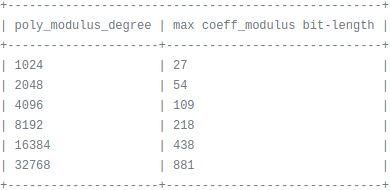
\includegraphics[width=0.5\linewidth]{images/Screenshot from 2021-10-05 23-37-47.png}
        \caption{Dependency between \texttt{coeff\_mod\_bit\_sizes} and \texttt{poly\_modulus\_degree} \href{https://github.com/microsoft/SEAL/blob/main/native/examples/1_bfv_basics.cpp}{Microsoft SEAL's Github Repository}}
        \label{fig:coeffpolytable}
    \end{figure} 
    
    In this lab, we chose these settings: 
        \begin{itemize}[nosep]
            \item[-] $\texttt{coeff\_mod\_bit\_sizes} = [37, 28, 28, 28, 28, 28, 28, 28, 37]$
            \item[-] $\texttt{poly\_mod\_degree} = 16384$
            \item[-] $\texttt{global\_scale} = 2^{28}$
        \end{itemize}
    Because we have a multiplicative depth of 7, the number list \texttt{coeff\_mod\_bit\_sizes} has a size of 9.
    
    With regard to sigmoid approximation, we decided to use $g_3$, because it needs a smaller depth for evaluation compared with $g_7$ (see figure \ref{fig:approxsigmoid}b). In addition, we did not use any other improved variant of Gradient Descent than just the original one.
    
    
    \begin{algorithm} \caption{logistic regression with the gradient descent to train CKKS-encrypted data}
    \label{code:pseudocode}
    \begin{algorithmic}[1]
        \Require $S$ - the CKKS-encrypted dataset consisting of $m$ tuples $(enc\_x, enc\_y)$, \linebreak $enc\_weight$ - initial weight vector consisting of 0s, $enc\_bias$ - initial bias with value of 0, $0 \leq lr \leq 1$ - learning rate 
        \While{$N \leq EPOCH\_count$}
            \ForEach {$(enc\_x, enc\_y) \in \mathcal S $}
                \State $\hat{y} \gets approximate\_sigmoid((enc\_x * enc\_weight) + enc\_bias)$
                \State $\Delta{w} \gets \Delta{w} + enc\_x * (\hat{y} - enc\_y)$
                \State $\Delta{b} \gets \Delta{b} + (\hat{y} - enc\_y)$
            \EndFor
        \State $enc\_weight \gets enc\_weight - lr * (\Delta{w}/m)$
        \State $enc\_bias \gets enc\_bias - lr * (\Delta{b}/m)$
        \State $\Delta{w} \gets 0$, $\Delta{b} \gets 0$
        \State $N \gets N + 1$
        \State \textbf{Bootstrapping}
        \EndWhile
    \State Return $enc\_weight$ and $enc\_bias$
    \end{algorithmic}
    \end{algorithm}
    An algorithm \ref{code:pseudocode} shows how we implement the logistic regression with the gradient descent to train CKKS-encrypted data. In line 11 of the algorithm \ref{code:pseudocode}, we need to bootstrap the $enc\_weight$ and $enc\_bias$, because our settings only allow  multiplicative depth 7. If we continue the while loop without bootstrapping, the information loss of the encrypted weights and the encrypted bias will increase drastically, which prevents information recovery. Since the TenSEAL library did not support bootstrapping in CKKS mode at the time of writing, we simulate the bootstrapping by decrypting the weights and the bias then encrypting them again.
    \subsection{Datasets}\marginnote{VTN}
    There are 4 datasets that are used to evaluate the experiments:
    \begin{itemize}[nosep]
        \item \hyperlink{https://www.kaggle.com/dileep070/heart-disease-prediction-using-logistic-regression}{\texttt{framingham}}: This dataset has 40000 rows, and 16 columns. Since we dropped some unrelated features and remove rows with missing values, only 1114 9-D datapoints were used to train a logistic regression model. The final model is to predict whether "10 year risk of coronary heart disease CHD" based on specific inputs is probable or not.
        \item \texttt{LogReg\_sample\_dataset}: This dataset is randomly generated. It has 1000 \linebreak 2-dimensional (2-D) datapoints. They are labeled with either 0 or 1, such that group of points with label 0 and group of points with label 1 are linearly separable. See definition of linear separability in definition \ref{def:linearseparability}.
        \item \texttt{HRF\_sample\_small}: This dataset is also randomly generated. It is linearly separable and it has 1000 5-D datapoints labeled with 0 or 1.
        \item \texttt{HRF\_samples\_big}: Similar to the dataset \texttt{HRF\_sample\_small}, it is linearly separable. However, it has 50000 5-D labeled with 0 or 1 datapoints.
    \end{itemize}
    \newtheorem{definition}{Definition}
    \begin{definition}
        Let $X_0$ and $X_1$ be 2 sets of points in an n-dimensional Euclidean space. Then $X_0$ and $X_1$ are \textit{linearly separable} if there exists $n+1$ real numbers $w_1, w_2,.., w_n, k$ such that every point $x \in X_0$ satifies $\sum_{i=1}^{n}w_ix_i > k$ and every point $x \in X_1$ satifies $\sum_{i=1}^{n}w_ix_i < k$, where $x_i$ is the $i$-th component of $x$.
        \caption{Definition of linear separability\cite{enwiki:1042160240}}
        \label{def:linearseparability}
    \end{definition}
    \subsection{Experiment Result}\marginnote{VTN}
    For each dataset, we use 70\% of the dataset to train, and the remaining 30\% of the dataset is used as a test set. The number of epochs is 100, each the training set is shuffled and fed to the algorithm with the learning rate is $0.01$.
    
    In table \ref{fig:encryptiontable}, we show the time to encrypt each dataset and the amount of memory to hold the encrypted datasets. We also should note that due to difference in matrix shape between original datasets and packed ones, we have to use different sets of $\texttt{poly\_mod\_degree}$ and $\texttt{coeff\_mod\_bit\_sizes}$ to make the encryption possible.  The table clearly shows that the time to encrypt the packed datasets and the amount of memory to hold the encrypted packed datasets are greatly smaller than the measurements of non-packed datasets. Because of the google colab's memory limitation, we could not encrypt the non-packed dataset \texttt{HRF\_samples\_big}, which has 50000 rows. As a result, we only use the first 2000 datapoints in the dataset \texttt{HRF\_samples\_big} to do the comparison. Another difficulty is that we could not train the encrypted-packed datasets, as the library TenSEAL had not supported vector shifting at the time of conducting the experiments.
    
    \begin{table}
    \resizebox{\textwidth}{!}{\begin{tabular}{ m{4cm} c c c c c c c c }
    \hline
    Dataset & Sample num & Feature num & Type & Parameter set & Encryption time (seconds) & Allocated memory \\
    \hline
    \multirow{3}{4em}{framingham} & \multirow{3}{4em}{1114} & \multirow{3}{4em}{9} & non-packed & Set 1 & 73.6 & 4.677 GB \\ 
    &&& packed & Set 2 & 0.145 & 0.0075 GB \\ 
    \hline
    \multirow{3}{4em}{LogReg\_sample\_dataset} & \multirow{3}{4em}{1000} & \multirow{3}{4em}{2} & non-packed & Set 1 & 64.5 & 4.197 GB \\ 
    &&& packed & Set 1 & 0.07 & 0.004 GB \\
    \hline
    \multirow{3}{4em}{HRF\_sample\_small} & \multirow{3}{4em}{1000} & \multirow{3}{4em}{5} & non-packed & Set 1 & 63.589 & 4.197 GB \\ 
    &&& packed & Set 1 & 0.067 & 0.0044 GB \\
    \hline
    \multirow{3}{4em}{HRF\_samples\_big} & \multirow{3}{4em}{first 2000 samples} & \multirow{3}{4em}{5} & non-packed & Set 1 & 136.2 & 8.39 GB \\ 
    &&& packed & Set 2 & 0.17 & 0.008 GB \\ 
    &&&&&\\
    \hline
    \end{tabular}}
    \caption{CKKS encryption time and allocated memory for 4 datasets. NOTE: Some packed datasets require a larger value of $\texttt{poly\_mod\_degree}$, so that we use 2 parameter sets: Set 1: $\texttt{poly\_mod\_degree} = 16384$, $\texttt{coeff\_mod\_bit\_sizes} = [37, 28, 28, 28, 28, 28, 28, 28, 37]$ \& Set 2: $\texttt{poly\_mod\_degree} = 32768$, $\texttt{coeff\_mod\_bit\_sizes} = [37, 28, 28, 28, 28, 28, 28, 28, 37]$.
    }
    \label{fig:encryptiontable}
    \end{table}
    
    Table \ref{fig:evaluationtable} not only tells the tiny differences between the final models trained by the CKKS logistic regression using the CKKS-encrypted data and the ones trained by the normal logistic regression using the original datasets, but also states the huge gaps of the runtime per epoch; because we do simulate bootstrapping process of CKKS during training the data, which also means the error produced by applying multiple multiplications on encrypted data is minimized. For the dataset \texttt{HRF\_samples\_big}, the out-of-memory error occurs during CKKS encryption process, which also stop the program from processing further to the learning step.
    
    \begin{table}
    \resizebox{\textwidth}{!}{\begin{tabular}{ m{4cm} c c c c c c c c }
    \hline
    Dataset & Sample num & Feature num & Method & Epoch num & seconds/epoch & Accuracy & Loss & Note\\
    \hline
    \multirow{3}{4em}{framingham} & \multirow{3}{4em}{1114} & \multirow{3}{4em}{9} & CKKS LR & 100 & 385 & 0.706 & 0.644 & \\ 
    &&& plaintext LR & 100 & 0.035 & 0.658 & 0.64 & \\ 
    \hline
    \multirow{3}{4em}{LogReg\_sample\_dataset} & \multirow{3}{4em}{1000} & \multirow{3}{4em}{2} & CKKS LR & 100 & 217 & 1.0 & 0.15 & \\ 
    &&& plaintext LR & 100 & 0.03 & 1.0 & 0.16 & \\ 
    \hline
    \multirow{3}{4em}{HRF\_sample\_small} & \multirow{3}{4em}{1000} & \multirow{3}{4em}{5} & CKKS LR & 100 & 303 &  0.89 & 0.31 & \\ 
    &&& plaintext LR & 100 & 0.33 & 0.89 & 0.30 & \\ 
    \hline
    \multirow{3}{4em}{HRF\_samples\_big} & \multirow{3}{4em}{50000} & \multirow{3}{4em}{5} & CKKS LR & 100 & X & X & X & Error: out of memory\\ 
    &&& plaintext LR & 100 & 0.78 & 0.89 & 0.32 & \\ 
    \hline
    \end{tabular}}
    \caption{CKKS LR implementation results for 4 datasets}
    \label{fig:evaluationtable}
    \end{table}
    
    In attempt to improve the runtime of the CKKS logistic regression's training process, we also try to apply concurrency programming pattern to the algorithm (section \ref{parallel}). Furthermore, we propose a way to reduce the memory needed to encrypt the data in section \ref{vectorization} in order to solve the out-of-memory problem we have in table \ref{fig:evaluationtable}.
    \section{Parallelization of learning}\label{parallel}\marginnote{GM}
\begin{text}
    \indent We've shown that learning on encrypted data which are encrypted with the CKKS scheme is possible. But it takes a long time to train the logistic regression. \newline
    \noindent The first attempt to speed up the learning process was to find a way to parallelize the calculation.

    $$\Delta w = \sum_{i<N} input_i \cdot (output_i-expected_i)$$

    \noindent With a look at the equation to calculate the weight changes during the learning process it is obvious where the approach is to split the equation for the threads. 
        
    $$\Delta w = \sum_{i=0}^{\frac{1}{T}N} input_i \cdot (output_i-expected_i) +...+\sum_{i=\frac{T-1}{T}N}^{N} input_i \cdot (output_i-expected_i)$$ 
    
    \noindent After splitting the sum into thread many sums we can calculate the partial sums in parallel and after this we need to sum up the pieces to get the whole sum. This should lead us to a speed up of learning. But we need to take care about some points if we work with threads.\newline
    \indent First of all we have only additions and multiplications, which are really fast calculations, in the threads. So we need to think about the overhead of threads. To create a thread some amount of time is needed. If the creation needs more time than the calculation then threading is not useful. But we can take care of the overhead if we use the busy waiting method where we start all needed threads at the beginning of our algorithm and the threads will never closed but they wait for information that they can work on. Here we need to know that all operating systems have an internal key how often a thread can be called in one second. If we create threads above our system kernels, then the operating system needs to set some threads to sleep. But if the down time of these threads is greater than the calculation time then too many threads will not help in a speed up. We should only use a number of threads equal to the number of kernels minus one for the calculation because the main process needs one thread too. Because the threads always run we need a global variable where we can tell the threads that new data are available and another global variable where the threads can tell that they are finished. So our main thread can tell the worker threads when they should work and our main thread knows when he can go on with his calculation. With these ideas we can create a workflow for the learning algorithm. The pseudo code in Algorithm \ref{workflow} shows this workflow. \newline
    
    \begin{algorithm} \caption{Workflow of learning}
        \label{workflow}
    	\begin{algorithmic}[1]
    	    \State{DECLARE GLOBAL $float$ weight $\gets 1.0$}
    	    \State{DECLARE GLOBAL $bool[]$ startFlag[threads] $\gets FALSE$}
    	    \State{DECLARE GLOBAL $float[]$ resultArray[threads]$\gets 0.0$}
    	    \State{DECLARE GLOBAL $bool[]$ doneArray[threads] $\gets FALSE$}
    	    \State
    	    \For{$i= 0$ to $(\#$threads$-1)$}
    	        \State{START thread $\gets$ \{i, ThreadFunction\}}
    	    \EndFor
    	    \State
    	    \While{$N \leq EPOCH\_count$}
                \State{doneArray $\gets FALSE$}
                \State{startFlag $\gets TRUE$} \Comment{Threads start calculation}
            	\State
        	    \While{True}
        	        \If{doneArray.ALL(TRUE)}
        	        \State{break} \Comment{Waiting for all threads are done}
        	        \EndIf
        	    \EndWhile
        	    \State
        	    \State $\Delta$ w = resultArray.SUM
        	    \State
        	    \State{weight $\gets$ weight + $\Delta$ w}
        	    \State
        	    \State $N \gets N + 1$
        	\EndWhile
    	\end{algorithmic}
    \end{algorithm}
    
    \indent Next we need to think about the single threads and how they should work and the calculation they should do. Because we will work with threads we need to think about race conditions and deadlocks of the threads. We have only one data set for all threads but the threads only need to read on this data set. So there is no problem. To avoid the race condition for the result we can use semaphores but then we maybe slow down the whole calculation because the threads need to wait. Better each thread has his own result and the main process sum up each single thread result after all threads are done with their calculation. For this we set up a global variable for the results. So we don't need semaphores and over all we have no race conditions and no deadlocks. We start each thread with a unique ID. This ID is the thread number, which starts with zero. With this ID we can specify on which data segment the thread should work.
    
    $$\text{starting point} = \frac{\text{ID}}{\text{number of threads}} \cdot \text{number of data points,}$$
    \newline
    $$\text{ending point} = \frac{\text{ID}+1}{\text{number of threads}} \cdot \text{number of data points.}$$
    \newline 
    \noindent We also use the ID to tell the thread the place where it can write his result and as an identification of the thread so the main thread knows which thread has finished. \newline
    \noindent Now, each thread needs to calculate his $\Delta$w on his data segment and need to wait until all other threads are done with their calculations and the main thread gives feedback to calculate another $\Delta$w for the next learning step. The pseudo code in Algorithm \ref{threadfunction} shows this thread function. \newline
    
    \begin{algorithm}
        \caption{ThreadFunction}
        \label{threadfunction}
    	\begin{algorithmic}[1]
    	    \State{$integer \text{\space threadID} \gets \text{i}$} \Comment{Given from main threat}
    	    \State{$integer \text{\space startPoint} =\left[\frac{\text{threadID}}{\#\text{threads}} \right]\cdot\#\text{dataPoints}$}
    	    \State{$integer \text{\space endPoint} = \left[\frac{\text{threadID}+1}{\#\text{threads}} \right]\cdot\#\text{dataPoints}$}
    	    \State{$float \text{\space result} \gets 0.0$}
    	    \State
    	    \While{$TRUE$}
                \State{startFlag[threadID] $\gets FALSE$ } \Comment{Global variable}
                \State
                \For{$i =$ startPoint \textbf{to} endPoint}
                    \State{result $+=$ input$_i * ($output$_i -$ expected$_i)$} \Comment{Calculating $\Delta$w from data segment}
                \EndFor
                \State
                \State{resultArray[threadID]$\gets$ result} \Comment{Global variable. Give result to main thread}
                \State{result$\gets 0.0$}
                \State{doneArray $\gets TRUE$} \Comment{Global variable. Tell main thread done}
                \State
                \While{$TRUE$}
                    \If{startFlag[threadID] $= TRUE$} \Comment{Global variable}
                        \State{break} \Comment{Waiting for start command}
                    \EndIf
                    \State{Do nothing}
                \EndWhile
        	\EndWhile
    	\end{algorithmic}
    \end{algorithm}
    
    \indent With this modifications we can do the training like in Algorithm \ref{code:pseudocode} but in parallel.  
    
    \subsection{Results and conclusions} \marginnote{GM}
    After several runs with different hardware set ups, we can't find a speed up for the calculations. By searching the web we found out that python has a global interpreter lock. This lock prevents multiple threads from executing codes at the same time. So the threads don’t run in parallel but linear. The multi threading lib still exist because with the lib the threads are executed more efficiently but not in parallel. \newline
    Instead of using multi threading we can use multi processing which python supports. But for this we need to think about the structure of our code because working with global variables isn't that easy like for multi threading. \newline
    Also we have a problem with the space requirements of the algorithm because we encrypt each data point individually. So we can maybe get a speed up by stacking data points before encryption and working with vector arithmetic. \newline
    So the parallelization is still an idea for big data sizes but not for smaller ones. 

\end{text}
    \section{Vectorization of data}\label{vectorization}\marginnote{GM}
\begin{text}
After the first attempt to make learning more efficient through parallelization, without any effect, we thought about vectorization of the data. For this we take a look at the encryption of data. The CKKS library gives us two options for the encryption. We can encrypt the data as vectors or as tensors. If we encrypt the input as tensors we can encrypt whole matrices in one step.
\end{text}

\subsection{Space requirements}\marginnote{GM}
\begin{text}
The first drawback of our idea for learning on encrypted data was the required space for the encrypted data. So we take a closer look on this topic. We used several matrices as inputs and encrypt them all with the same CKKS context that we have used so far. In the table of figure \ref{fig:baseline} we can see how many megabyte are used for the encryption of $m$ data points with dimension $n$ where we encrypted each single data point with one CKKS vector. These results are our baseline to see if we can find better ways to encrypt a whole data set.
\end{text}

\begin{figure}[ht]
\centering
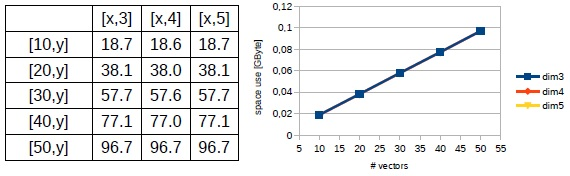
\includegraphics[width=1\linewidth]{images/baseline.jpg}
\caption{Space requirements of encrypted $[m\times n]$-matrices as vectors row by row in megabyte.}
\label{fig:baseline}
\end{figure} 

\begin{text}
With the graph of figure \ref{fig:baseline} we can easily see that the dependency on dimension of the data points is not measurable for our small dimensions and that the encryption of multi vectors is linear. \newline
\indent Next, we measure the space requirements of CKKS tensors. We use the same context and the input arrays like before but now we encrypt the whole $m$ data points with dimension $n$ with only one CKKS tensor. The idea is that the CKKS scheme can encrypt multiple data points more efficient as a CKKS tensor by its own than we do before. In the table of figure \ref{fig:tensor} we can see how many megabyte are used for the encryption.
\end{text}

\begin{figure}[ht]
\centering
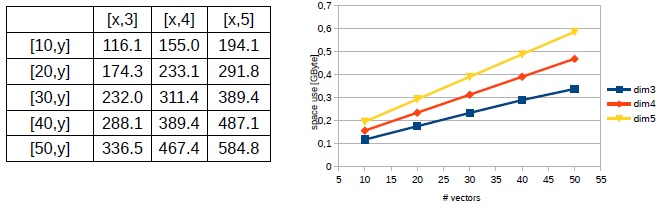
\includegraphics[width=1\linewidth]{images/tensor.jpg}
\caption{Space requirements of encrypted $[m\times n]$-matrices as one tensor in megabyte.}
\label{fig:tensor}
\end{figure} 

\begin{text}
With the graph of figure \ref{fig:tensor} we can see that the dimension of the data points has an impact. Higher dimension use more space than lower dimension and over all the space requirements are much more than the encryption row by row. So the encryption as a CKKS tensor doesn't solve the space requirement problem we have. \newline
From the results of the measurements of the baseline that the dependency on dimension of the data points is not measurable for our small dimensions we try to find a limit where we see a dependency on dimension. For this we flatten the matrix in such a way that we have only a vector with a dimension of m times n.We encrypt this vector with the same context like before.
\end{text}

\begin{figure}[ht]
\centering
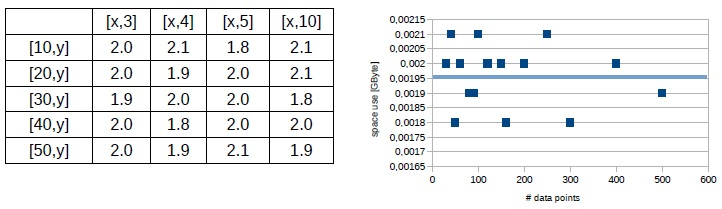
\includegraphics[width=1\linewidth]{images/flatten.jpg}
\caption{Space requirements of encrypted flatten $[m\times n]$-matrices as vector in megabyte.}
\label{fig:flatten}
\end{figure} 

\begin{text}
In figure \ref{fig:flatten} we can see that the flatten matrix use nearly the same space for each vector independent of the dimension at least for our data range. So we can handle the high space requirement of our algorithm if we use flatten matrices as an input and we can find a way to calculate with such a flatten matrix.
\end{text}

\subsection{Calculation with vectorized data}\marginnote{GM}
\begin{text}
Let's assume that all users stores their encrypted data points as a struc where you know the dimension $n$ of the data points and the number $m$ of data points that are encrypted. Maybe you need the context how the data points are encrypted and at least the encrypted data points as a vector. Figure \ref{fig:vec} a) shows an example of such an vectors. In the example $x_{m,1}$ and $x_{m,2}$ are the coordinates of the 2-dimensional data points, $b_m$ is the bias that is usually set to 1 and $y_m$ is the expected output. With this struc we are going to create another vector, a weight vector. The size of the weight vector is the same size like the data vector. Figure \ref{fig:vec} b) shows an example of such a weight vector. In the example we have a sub sequence of two weights $w_1$ and $w_2$ to weight the coordinates, another weight $w_b$ to wight the bias followed by a $1$. This sub sequence is repeated $m$ times in the whole weight vector. \newline

\begin{figure}[ht]
    \centering
    \begin{tabular}{c|c|c|c|c|c|c|c|c|c|c|c|c|c}
        \cline{2-13}
        a) & $x_{1,1}$ & $x_{1,2}$ & $b_{1}$ & $y_{1}$ & $x_{2,1}$ & $x_{2,2}$ & $b_{2}$ & $y_{2}$ & $x_{3,1}$ & $x_{3,2}$ & $b_{3}$ & $y_{3}$ & $\dots$  \\
        \cline{2-13}
        \noalign{\medskip}
        \cline{2-13}
        b) & $w_1$ & $w_2$ & $w_b$ & $1$ & $w_1$ & $w_2$ & $w_b$ & $1$ & $w_1$ & $w_2$ & $w_b$ & $1$ & $\dots$  \\
        \cline{2-13}
    \end{tabular}
    \caption{a) Encrypted data point vector. b) Weight vector}
    \label{fig:vec}
\end{figure}

After the encryption of the weight vector we can replace the for loop to calculate $\Delta$w in our algorithm \ref{threadfunction} with simple vector arithmetic. We multiply the encrypted data point vector point-wise with the weight vector. The resulting vector together with the data point vector includes all values we need to calculate $\Delta$w. Figure \ref{fig:resvec} illustrates this calculation. \newline

\begin{figure}[ht]
    \centering
    \begin{tabular}{|c|c|c|c|c|c|c|c|c|c|c|c|c}
        \cline{1-12}
        $x_{1,1}$ & $x_{1,2}$ & $b_{1}$ & $y_{1}$ & $x_{2,1}$ & $x_{2,2}$ & $b_{2}$ & $y_{2}$ & $x_{3,1}$ & $x_{3,2}$ & $b_{3}$ & $y_{3}$ & $\dots$  \\
        \cline{1-12}
        \noalign{\smallskip}
        \multicolumn{13}{c}{point-wise multiplication} \\
        \noalign{\smallskip}
        \cline{1-12}
        $w_1$ & $w_2$ & $w_b$ & $1$ & $w_1$ & $w_2$ & $w_b$ & $1$ & $w_1$ & $w_2$ & $w_b$ & $1$ & $\dots$  \\
        \cline{1-12}
        \noalign{\smallskip}
        \multicolumn{13}{c}{$=$} \\
        \noalign{\smallskip}
        \cline{1-12}
        $w_1 x_{1,1}$ & $w_2 x_{1,2}$ & $w_b b_{1}$ & $y_{1}$ & $w_1 x_{2,1}$ & $w_2 x_{2,2}$ & $w_b b_{2}$ & $y_{2}$ & $w_1 x_{3,1}$ & $w_2 x_{3,2}$ & $w_b b_{3}$ & $y_{3}$ & $\dots$  \\
        \cline{1-12}    
    \end{tabular}
    \caption{Calculation of the resulting vector}
    \label{fig:resvec}
\end{figure}

To calculate $\Delta$w we need the output, the expected output and the input. With an encrypted selection vector we are able to choose parts from the data point and resulting vector we need. Figure \ref{fig:chovec} shows an example where we select the parts of the resulting vector that we need to approximate the output of the neuron with the first data point as input.

\begin{figure}[ht]
    \centering
    \begin{tabular}{|c|c|c|c|c|c|c|c|c|c|c|c|c}
        \cline{1-12}
        $w_1 x_{1,1}$ & $w_2 x_{1,2}$ & $w_b b_{1}$ & $y_{1}$ & $w_1 x_{2,1}$ & $w_2 x_{2,2}$ & $w_b b_{2}$ & $y_{2}$ & $w_1 x_{3,1}$ & $w_2 x_{3,2}$ & $w_b b_{3}$ & $y_{3}$ & $\dots$  \\
        \cline{1-12}
        \noalign{\smallskip}
        \multicolumn{13}{c}{dot product} \\
        \noalign{\smallskip}
        \cline{1-12}
        $1$ & $1$ & $1$ & $0$ & $0$ & $0$ & $0$ & $0$ & $0$ & $0$ & $0$ & $0$ & $\dots$  \\
        \cline{1-12}
        \noalign{\smallskip}
        \multicolumn{13}{c}{$=$} \\
        \noalign{\smallskip}
        \multicolumn{13}{c}{$w_1 x_{1,1} + w_2 x_{1,2} + w_b b_{1}$} \\
    \end{tabular}
    \caption{Selection of the results for the first data point as input.}
    \label{fig:chovec}
\end{figure}

To the result of the selection in figure \ref{fig:chovec} we can now apply the approximation of the sigmoid function to get the output. With a different selection vector we can choose the corresponding expected output like before. With another selection vector we need to select the corresponding data point. Now we are able to use the calculation of $\Delta$w from our algorithm \ref{code:pseudocode}. \newline
If we use the selection vectors for each data point we can run our algorithm for learning with encrypted vectors. But to get a speed up by using vectors we need to use matrix multiplications instead of vector multiplications because otherwise we replace one for loop with another. But for now matrix multiplications in the CKKS scheme is still missing.
\end{text}
    \section{Summary and outlook}\marginnote{GM}
\begin{text}
We could show that logistic regression and learning on CKKS encrypted data is possible. We found some drawbacks with space requirements and learning speed. And without bootstrapping for encrypted data we need to send data back to do bootstrapping on user side. \newline
We found a way for parallelization but in future work we need to rebuild the algorithm to fit with python. We can't use multi-threading but we need to use multi-processing. \newline
With the vectorization we have an idea to handle the drawback of space requirements and also the speed up of learning. Unfortunately the CKKS scheme has no matrix operations implemented yet, so we need to build our own library in future work to prove our ideas of vectorization with respect to space requirements and speed up. \newline
As another programming task for the future we need bootstrapping on encrypted data to get security. Here we need to wait that bootstrapping is given to the software we used or we need to implement one.\newline
After the programming tasks are done we need to think about the security of our algorithm and how secure we are and maybe how we can increase the security level if necessary.
Finally, we need to think about how data points from various sources can come together to generate a training data pool. Here we can use our idea of parallelization but to run this efficient we need to change from python to C++ as our programming language.
\end{text}
    \newpage
    \printbibliography[heading={bibintoc}, title={\hspace*{6mm}References}]
\end{document}